\renewcommand{\nomebreve}{bridges\_and\_cutnodes}
\renewcommand{\titolo}{Ponti e nodi di articolazione in grafi non diretti}

\introduzione{}

\noindent
Il tuo programma riceve in input un grafo  $G=(V,E)$ \emph{non-diretto}\footnote{{\bf non-diretto:} su nessun arco è imposta una direzione, ossia gli archi rappresentano tutti strade a doppio senso di circolazione.}, connesso\footnote{{\bf connesso:} per ogni due nodi esiste un cammino che li congiunge.}, e semplice\footnote{{\bf semplice:} non contiene nè loops (un loop è un arco i cui estremi coincidono) nè archi paralleli (due archi sono paralleli se congiungono la stessa copia di nodi).}.\\
\indent
Un arco $e\in E$ si dice un \emph{ponte} (o \emph{bridge}) di $G$ se il grafo che si ottiene da $G$ con la rimozione di $e$ non è più connesso.\\
\indent
Un nodo $v\in V$ si dice un \emph{nodo di articolazione} (o \emph{cutnode}) di $G$ se il grafo che si ottiene da $G$ con la rimozione di $v$ non è più connesso.


\begin{figure}[h!]
\begin{center}
  \noindent 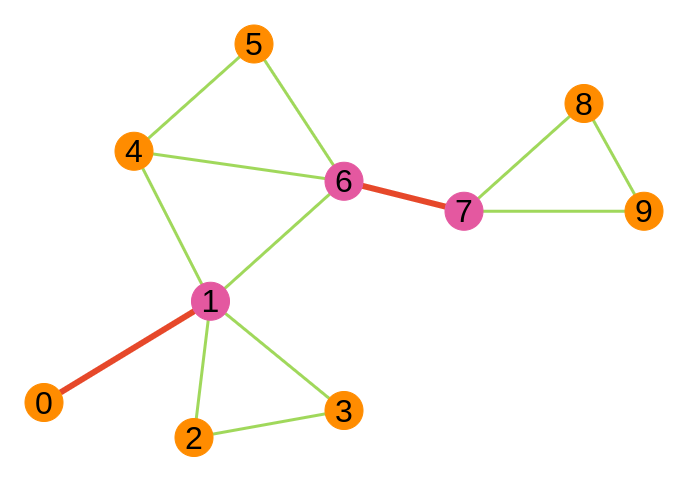
\includegraphics[width=0.45\textwidth]{figures/bridges_and_cutnodes.png}
\end{center}
\caption{Bridges in rosso e cutnodes in viola.}
\end{figure}


Vogliamo valutare e consentire l'espressione delle seguenti competenze:
\begin{description}
\item[subtask di tipo~$t=1$] saper identificare quali archi siano dei bridge;
\item[subtask di tipo~$t=2$] saper identificare quali nodi siano dei cutnode;
\item[subtask di tipo~$t=3$] specificare per ogni nodo $v$ quante siano le componenti connesse del grafo ottenuto da $G$ per rimozione del nodo $v$. Se intendi fornire una soluzione lineare anche per questo tipo di subtask allora potrebbe convenirti acquisire la nozione di componente biconnessa esposte nella sezione di appendice. 
\end{description}


\sezionetesto{Input ed Output}

Input ed output avvengono da \verb'stdin' e su \verb'stdout' rispettivamente.
La prima riga dell'input contiene i tre numeri $t$, $n$ ed $m$, nell'ordine e separati da spazio. Il numero $t$ indica la richiesta come da tabella sopra, mentre $n:=|V|$ e $m:=|E|$. Per rappresentare $G$, i nodi in $V$ sono messi in corrispondenza biunivoca coi numeri naturali da~$0$ a~$n-1$.
Seguono $m$ righe dove ciascuna riga codifica un diverso arco $e=uv\in E$ riportandone gli estremi. In pratica, dove assumiamo $u < v$, la riga contiene i due numeri $u$ e $v$, nell'ordine, e separati da spazio.
Queste $m$ righe sono date in ordine lessicografico (si vedano gli esempi).

\indent
Per subtask di tipo $t=1$ l'output consta di $m$ cifre binarie stampate una per riga. L'$i$-esima di queste cifre è $1$ se l'$i$-esimo arco letto in input è un bridge di $G$, altrimenti è $0$.\\
\indent
Per subtask di tipo $t=2$ l'output consta di $n$ cifre binarie stampate una per riga. L'$i$-esima di queste cifre è $1$ se il nodo $(i-1)$ è un cutnode di $G$, altrimenti è $0$.\\
\indent
Per subtask di tipo $t=3$ l'output consta di $n$ numeri interi positivi stampati uno per riga. L'$i$-esimo di questi numeri è il numero di componenti biconnesse che contengono il nodo $i$. 


% Esempi
\sezionetesto{Esempio di input/output}

In attachment alla pagina del problema trovate diverse coppie input/output tra cui le seguenti.

\vspace{0.5cm}
\esempio{1 10 13

0 1
  
1 2

1 3

1 4

1 5

1 6

2 3

4 5

5 6

6 7

7 8

7 9

8 9}{1
  
0
  
0

0

0

0

0

0

0

1

0

0

0}

\vspace{0.5cm}
\esempio{2 10 13
  
0 1
  
1 2

1 3

1 4

1 5

1 6

2 3

4 5

5 6

6 7

7 8

7 9

8 9}{0
  
1

0

0

0

0

1

1

0

0}

\vspace{0.5cm}
\esempio{3 10 13 10

0 1
  
1 2

1 3

1 4

1 5

1 6

2 3

4 5

5 6

6 7

7 8

7 9

8 9}{1
  
3
  
1

1

1

1

2

2

1

1}

\sezionetesto{Appendice: Struttura delle componenti biconnesse}

Per chi voglia affrontare anche il terzo tipo si subtask (non offre tanti punti, valuta dove investire il tuo tempo), aggiungiamo qui qualche ulteriore concetto (che non aiuta per i primi due tipi di subtask).
Dove $S\subseteq V$ è un insieme di nodi, denotiamo con $G[S]$ il \emph{sottografo di $G$ indotto da $S$}, ossia il grafo che si ottiene da $G$ per rimozione dei nodi in $V\setminus S$.   
Un grafo senza cutnodes è detto \emph{biconnesso}. Le \emph{componenti biconnesse} (o \emph{blocchi}) di $G$ sono quei sottoinsiemi $B\subseteq V$ massimali per cui $G[B]$ è biconnesso.

Sia $\mathcal{B}$ l'insieme di blocchi di $G$ e $C$ l'insieme dei cutnodes.
L'albero delle componenti biconnesse di $G$, indicato con $T_G$, ha per nodi gli elmenenti dell'insieme $\mathcal{B}\cup C$ ed è bipartito coi nodi di $\mathcal{B}$ da un lato e i nodi di $C$ dall'altro. Un cutnode $v\in C$ è adiacente ad un blocco $B\in \mathcal{B}$ se e solo se $v\in B$.  


\begin{figure}[h!]
\begin{center}
  \noindent 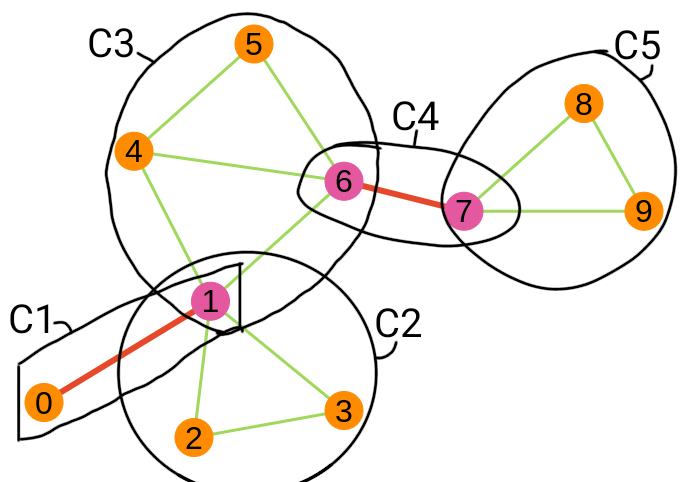
\includegraphics[width=0.40\textwidth]{figures/biconnected_components.png} \hfill 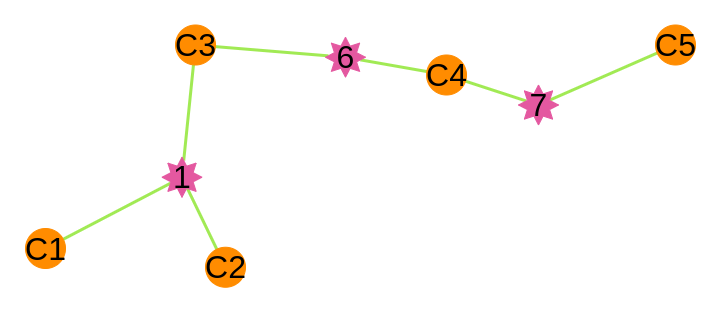
\includegraphics[width=0.40\textwidth]{figures/biconnected_components_tree.png}
\end{center}
\caption{Le componenti biconnesse e la loro struttura ad albero.}
\end{figure}


% Assunzioni
%\sezionetesto{Assunzioni e note}
%\begin{itemize}[nolistsep, noitemsep]
%  \item $1 \le n \le 100\,000$.
%\end{itemize}

\section*{Subtask}

  \begin{itemize}
    \item \textbf{Subtask 1 [0 punti]:} i casi di esempio forniti alla pagina del problema, essi includono i due casi sopra.
    \item \textbf{Subtask 2 [ 7 punti]:} $t=1$, $n \le 20$, $m \le 100$.
    \item \textbf{Subtask 3 [ 8 punti]:} $t=1$, $n \le 1000$, $m \le 10\,000$.
    \item \textbf{Subtask 4 [17 punti]:} $t=1$, $n \le 50\,000$, $m \le 200\,000$.
    \item \textbf{Subtask 5 [ 8 punti]:} $t=2$, $n \le 20$, $m \le 100$.
    \item \textbf{Subtask 6 [ 8 punti]:} $t=2$, $n \le 1000$, $m \le 10\,000$.
    \item \textbf{Subtask 7 [17 punti]:} $t=2$, $n \le 50\,000$, $m \le 200\,000$.
    \item \textbf{Subtask 8 [ 9 punti]:} $t=3$, $n \le 20$, $m \le 100$.
    \item \textbf{Subtask 9 [ 9 punti]:} $t=3$, $n \le 1000$, $m \le 10\,000$.
    \item \textbf{Subtask 10 [17 punti]:} $t=3$, $n \le 50\,000$, $m \le 200\,000$.
  \end{itemize}
  
